%!TEX TS-program = xelatex  
%!TEX encoding = UTF-8 Unicode  

\documentclass[12pt]{article}  
\usepackage{geometry}  
\geometry{letterpaper}  
\usepackage{fancyhdr}
\usepackage{extramarks}
\usepackage{amsmath}
\usepackage{amsthm}
\usepackage{amsfonts}
\usepackage{tikz}
\usepackage[plain]{algorithm}
\usepackage{algpseudocode} 
\usepackage{caption}
\usepackage{booktabs}
\usepackage{graphics}
\usepackage{amsmath}
\usepackage{amsfonts}

\usepackage{xltxtra,fontspec,xunicode}
\usepackage[slantfont,boldfont]{xeCJK}
\setCJKmainfont{宋体}   
\setmainfont{Optima}   
\defaultfontfeatures{Mapping=tex-text}  

\usepackage{xltxtra,fontspec,xunicode}
\usepackage[slantfont,boldfont]{xeCJK}
\setCJKmainfont{宋体}   
\setmainfont{Optima}   
\defaultfontfeatures{Mapping=tex-text}  

\XeTeXlinebreaklocale “zh”  
\XeTeXlinebreakskip = 0pt plus 1pt minus 0.1pt   
 
\usepackage{listings}
\usepackage{color}
\definecolor{dkgreen}{rgb}{0,0.6,0}
\definecolor{gray}{rgb}{0.5,0.5,0.5}
\definecolor{mauve}{rgb}{0.58,0,0.82}

\lstset{frame=tb,
  language=Java,
  aboveskip=3mm,
  belowskip=3mm,
  showstringspaces=false,
  columns=flexible,
  basicstyle={\small\ttfamily},
  numbers=none,
  numberstyle=\tiny\color{gray},
  keywordstyle=\color{blue},
  commentstyle=\color{dkgreen},
  stringstyle=\color{mauve},
  breaklines=true,
  breakatwhitespace=true,
  tabsize=3
} 

\topmargin=-0.45in
\evensidemargin=0in
\oddsidemargin=0in
\textwidth=6.5in
\textheight=9.0in
\headsep=0.25in

\linespread{1.1}

\pagestyle{fancy}
\lhead{\hmwkAuthorName}
\rhead{\hmwkClass}
\chead{\hmwkTitle}

\renewcommand\headrulewidth{0.4pt}
\renewcommand\footrulewidth{0.4pt}

\setlength\parindent{0pt}

% Homework Details

\newcommand{\hmwkTitle}{homework\ \#3}
\newcommand{\hmwkClass}{Deep Reinforcement Learning}
\newcommand{\hmwkAuthorName}{Tianxiao Hu}


\begin{document}
\pagebreak

\section{Q-Learning}
\subsection{basic Q-learning performance}
\begin{figure}[!h]
\centering
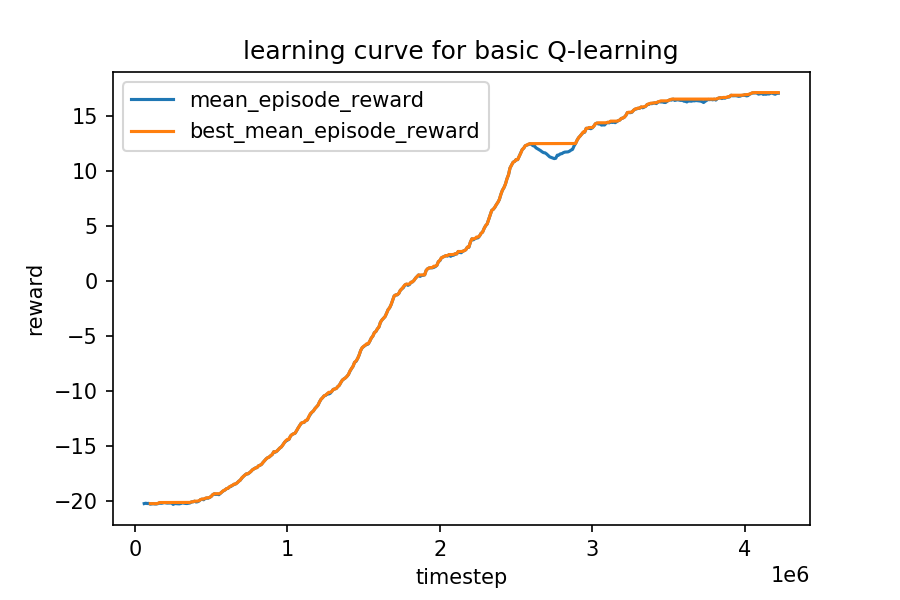
\includegraphics[width=4.2in]{Figure_1.png}
\caption{Learning curve for basic Q-learning, 4.2m time steps were trained on \textit{Atari} task.}
\end{figure}

\subsection{double Q-learning}
\begin{figure}[!h]
\centering
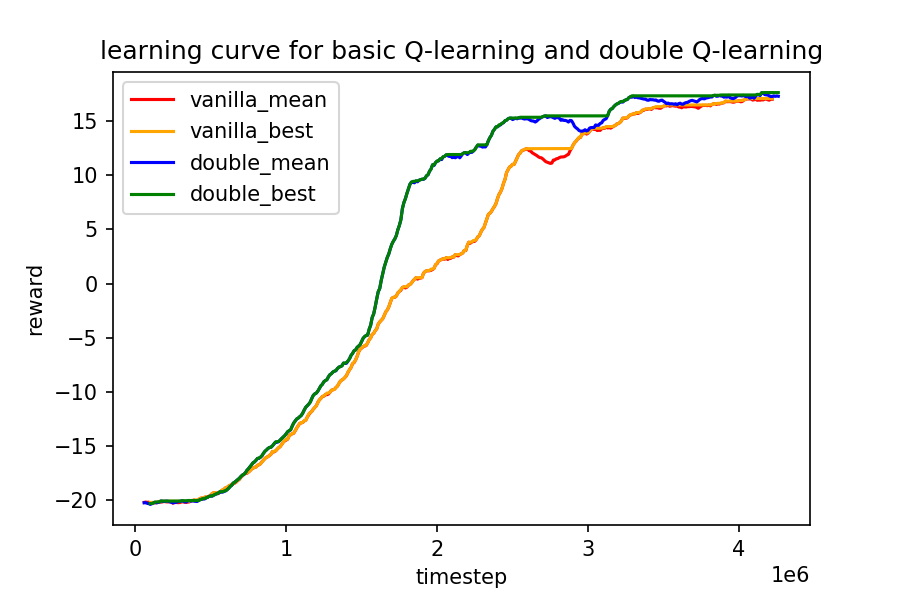
\includegraphics[width=4.2in]{Figure_2.png}
\caption{Learning curve for basic Q-learning vs double Q-learning, 4.2m time steps were trained on \textit{Atari} task.}
\end{figure}

\subsection{double Q-learning}
\begin{figure}[!h]
\centering
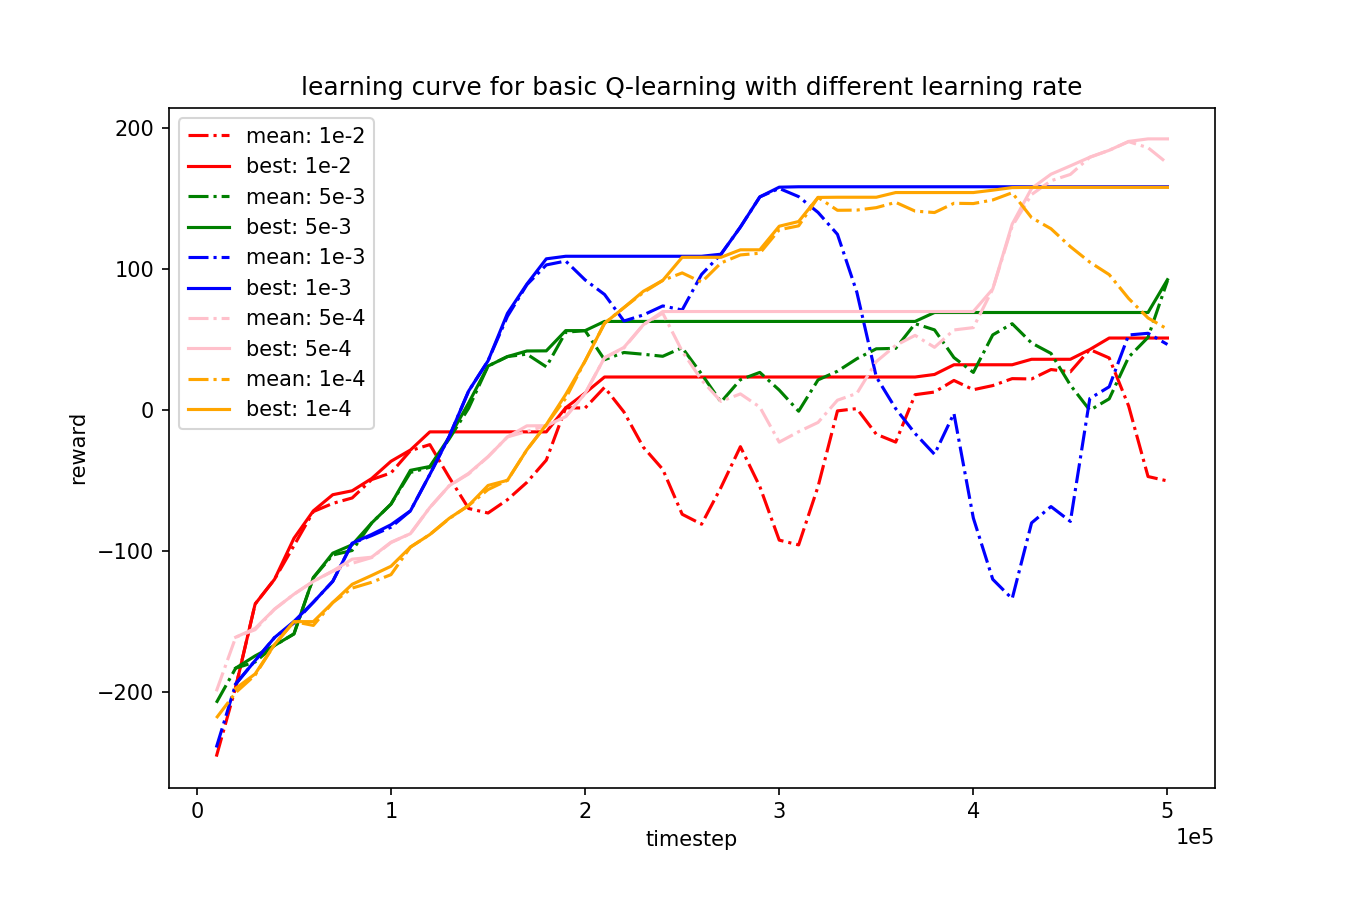
\includegraphics[width=6in]{Figure_3.png}
\caption{Learning curve for basic Q-learning with different learning rates, 50k time steps were trained on \textit{lunar lander} task. I choose the learning rate parameter to evaluate the sensitivity to hyper-parameters of the algorithm. Typically, larger learning rate fasten the convergence, but it is easy to jump out of a good local minima and finally make the agent fall into a terrible place. Small learning rates requires more iteration to get to a convergence, but the training procedures are more stable, which results in better performance. However, the performance varies in different tasks. So choosing a good learning rate is important in many RL tasks.}
\end{figure}

\newpage
\section{Actor-Critic}
\subsection{Sanity check with Cartpole}
\begin{figure}[!h]
\centering
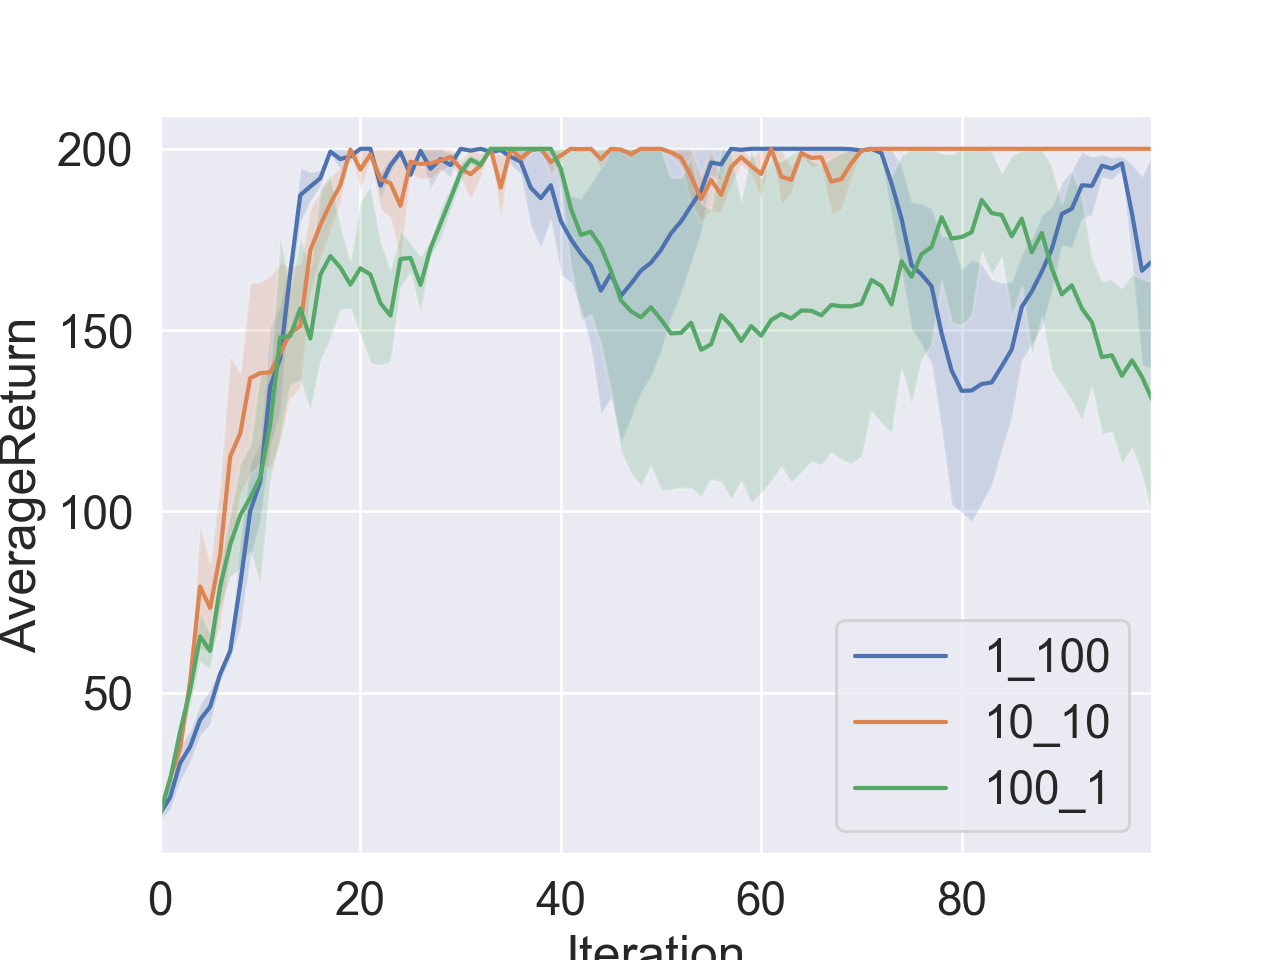
\includegraphics[width=4in]{Figure_4.png}
\caption{Learning curve for \textit{Cartpole} task with different hyperparameters. From the plot, we can see (10, 10) is the best parameter set for it converges quickly and more stable compared to (1, 100).}
\end{figure}

\subsection{Run actor-critic with more difficult tasks}
\begin{figure}[!h]
\centering
\begin{minipage}[t]{0.48\textwidth}
\centering
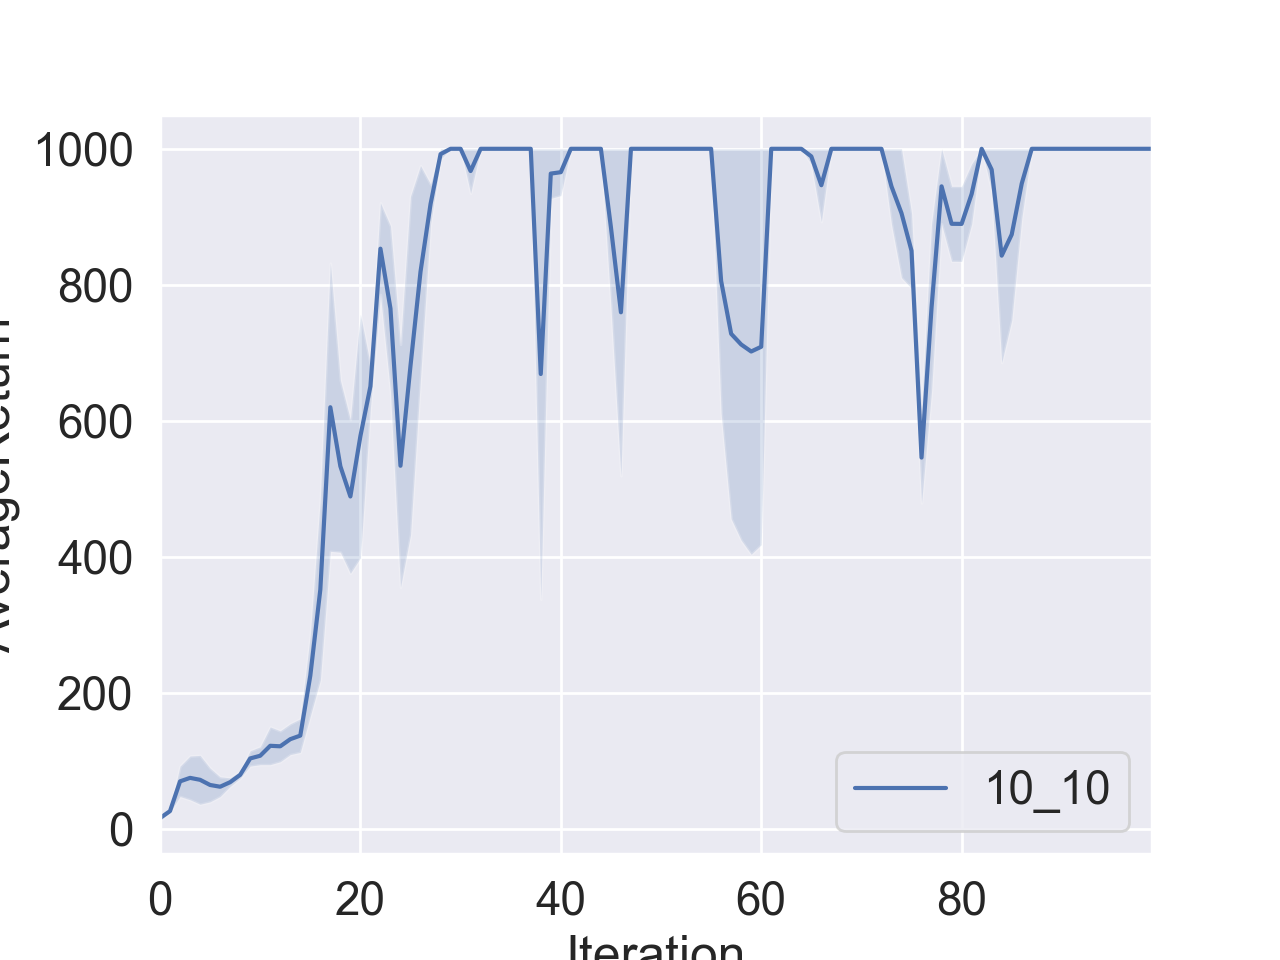
\includegraphics[width=8cm]{Figure_5.png}
\caption{Learning curve for \textit{InvertedPendulum} task.}
\end{minipage}
\begin{minipage}[t]{0.48\textwidth}
\centering
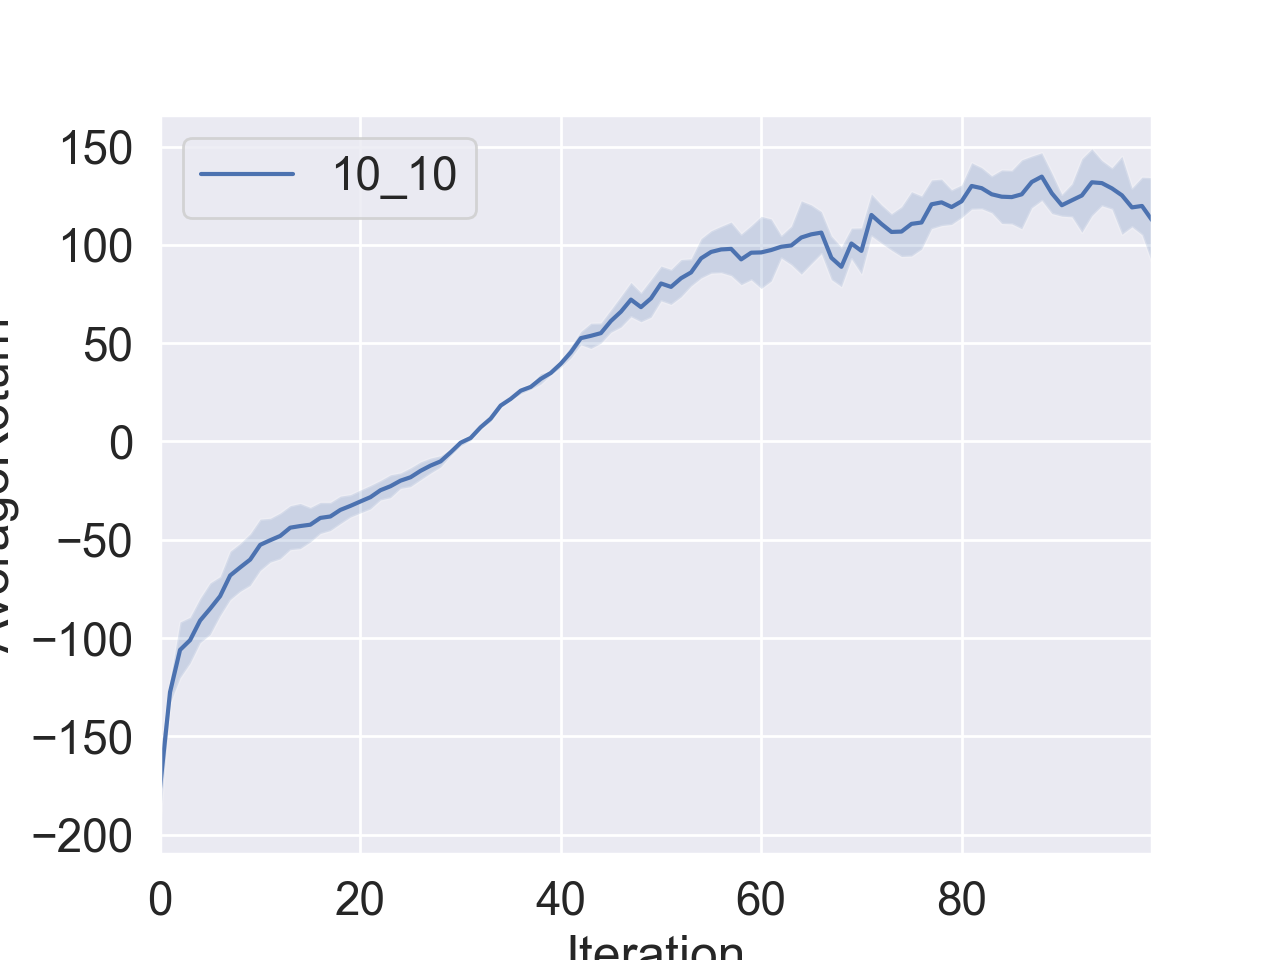
\includegraphics[width=8cm]{Figure_6.png}
\caption{Learning curve for \textit{HalfCheetah} task.}
\end{minipage}
\end{figure}

\end{document}  
  